\documentclass[11pt]{article}
\usepackage{latexsym}
\usepackage{amsmath,amssymb,amsthm}
\usepackage{epsfig}
\usepackage{float}
\usepackage{enumerate}
\usepackage{booktabs}
\usepackage{graphicx}
\usepackage[right=0.8in, top=1in, bottom=1.2in, left=0.8in]{geometry}
\usepackage{setspace}
\usepackage{subfigure}
\usepackage[ruled,linesnumbered]{algorithm2e}  
\usepackage{amsmath}
\usepackage{indentfirst} 
%\setlength{\parindent}{2em}
\usepackage{hyperref}
% comma: 用逗号分隔多个引用; square:使用方括号; super:引用是上角标形式
\usepackage[comma,square,super]{natbib}
\spacing{1.06}
\usepackage{titlesec}
\titleclass{\subsubsubsection}{straight}[\subsection]

\newcounter{subsubsubsection}[subsubsection]
\renewcommand\thesubsubsubsection{\thesubsubsection.\arabic{subsubsubsection}}
\renewcommand\theparagraph{\thesubsubsubsection.\arabic{paragraph}}

\titleformat{\subsubsubsection}
{\normalfont\normalsize\bfseries}{\thesubsubsubsection}{1em}{}
\titlespacing*{\subsubsubsection}
{0pt}{3.25ex plus 1ex minus .2ex}{1.5ex plus .2ex}

\makeatletter
\renewcommand\paragraph{\@startsection{paragraph}{5}{\z@}%
	{3.25ex \@plus1ex \@minus.2ex}%
	{-1em}%
	{\normalfont\normalsize\bfseries}}
\renewcommand\subparagraph{\@startsection{subparagraph}{6}{\parindent}%
	{3.25ex \@plus1ex \@minus .2ex}%
	{-1em}%
	{\normalfont\normalsize\bfseries}}
\def\toclevel@subsubsubsection{4}
\def\toclevel@paragraph{5}
\def\toclevel@paragraph{6}
\def\l@subsubsubsection{\@dottedtocline{4}{7em}{4em}}
\def\l@paragraph{\@dottedtocline{5}{10em}{5em}}
\def\l@subparagraph{\@dottedtocline{6}{14em}{6em}}
\makeatother

\setcounter{secnumdepth}{4}

\newcommand{\handout}[5]{
  \noindent
  \begin{center}
  \framebox{
    \vbox{\vspace{0.25cm}
      \hbox to 5.78in { {SE3352:\hspace{0.12cm}Algorithm Design} \hfill #2 }
      \vspace{0.48cm}
      \hbox to 5.78in { {\Large \hfill #5  \hfill} }
      \vspace{0.42cm}
      \hbox to 5.78in { {#3 \hfill #4} }\vspace{0.25cm}
    }
  }
  \end{center}
  \vspace*{4mm}
}
\newcommand{\lecture}[4]{\handout{#1}{#2}{#3}{Scribes:\hspace{0.08cm}#4}{Notes #1}}

\newtheorem{theorem}{Theorem}
\newtheorem{corollary}[theorem]{Corollary}
\newtheorem{lemma}[theorem]{Lemma}
\newtheorem{observation}[theorem]{Observation}
\newtheorem{example}[theorem]{Example}
\newtheorem{definition}[theorem]{Definition}
\newtheorem{claim}[theorem]{Claim}
\newtheorem{fact}[theorem]{Fact}
\newtheorem{assumption}[theorem]{Assumption}
\newcommand{\E}{\textbf{E}}
\newcommand{\var}{\text{var}}
\def\eps{\ensuremath\epsilon}
\begin{document}
\setlength{\parindent}{2em}

\lecture{1 -- Reachability on Large-scale Graphs}{\today}{Instructor:\hspace{0.08cm}\emph{Guoqiang Li}}{\emph{Zihong Lin}}


\section{Introduction}
The notes will focus on the reachability on large-scale graphs(hereinafter to be referred as 'reachability problem'). Many physical systems and items can be abstracted into a graph. Naturally, we can abstract the relationship network into a graph(The vertices are the people, while the edges are the relationship between people. Commonly, we can abstract 'a knows b' into $a\rightarrow b$). In modern application scenarios, the graph is usually large-scale. So research on the reachability problems is very meaningful.

\section{Problem description}
\begin{definition}
	[Reachable]
	Let $G=(V,E)$ be a directed graph.
	For any two vertices $u,v\in{V}$, if there exists a path from $u$ to $v$, we say $v$ is \textbf{reachable} from $u$, denoted as $u\rightarrow v$.
\end{definition}
\begin{definition}
	[Reachability problem]
	Given a directed graph $G=(V,E)$ and a pair of vertices $u,v\in{V}$, \textbf{the reachability problem} is to decide whether $u\rightarrow v$, and return TRUE or FALSE accordingly.
\end{definition}
\section{Algorithms/Models}
The algorithms of reachability problem can be further subdivided into index-based and index-free algorithms. Table \ref{table:algorithms}\cite{ref1} shows some of the mainstream algorithms.
Unless otherwise specified, we refer $n$ as the number of nodes(vertices) and $m$ as the number of edges.
\begin{table}[H]
	\centering
	\caption{\newline \ The mainstream algorithms on graph reachability.}
	\begin{tabular}{l|l|l|l}
		\toprule
		Method & Query Time & Construction & Index Size \\ \midrule
		DFS/BFS&  $O(n+m)$   &$O(n+m)$      &$O(n+m)$    \\ \midrule
		Transitive Closure&   $O(1)$      & $O(nm)=O(n^3)$     & $O(n^2)$ \\ \midrule
		Optimal Tree Cover
		(Agrawal et al., SIGmOD’89)& $O(n)$  &$O(nm)=O(n^3)$     &$O(n^2)$            \\ \midrule
		GRIPP
		(Tri$\beta$l et al., SIGMOD’07)&  $O(m-n)$&$O(n+m)$ &$O(n+m)$ \\ \midrule
		Dual-Labeling
		(Wang et al., ICDE’06)& $O(1)$ &$O(n+m+t^3)$&$O(n+t^2)$ \\ \midrule
		Optimal Chain Cover 
		(Jagadish, TODS’90)&$O(k)$ &$O(nm)=O(n^3)$&$O(nk)$  \\ \midrule
		2-HOP (SODA 2002) &$O(nm^{1/2})$&$O(n^3|T_C|)=O(n^5)$&$O(m^{1/2})$ \\ \midrule
		3-HOP 
		(Yang Xiang et al., SIGMOD ‘09)&$O(log n +k)$  &$O(kn^2)$&$O(nk)$\\ \bottomrule
	\end{tabular}
	\label{table:algorithms}
\end{table}
\subsection{Index-based algorithm}
The reachability index is a summary of all or part of the reachability information on the graph obtained by pre-computing the graph before querying (all reachability information is the information about whether any pair of vertex is reachable). Unless otherwise specified, the accessibility index so far is calculated based on the directed acyclic graph extracted from the original graph, rather than directly calculated from the original graph.

Specifically, this kind of directed acyclic graph compresses each strongly connected component in the original directed graph into a super node(vertex). If there is a node in one strongly connected component pointing to another strongly connected component, then connect the edges between the corresponding two super nodes. This method of compressing the original digraph can obviously save its reachability information losslessly: the two nodes are reachable if and only if they are reachable between the super nodes to which they belong.  At the same time, this method can reduce the space overhead of the index, and the structural characteristics of the directed acyclic graph also make the establishment of some indexes easier, so it is widely used.

\begin{definition} 	[Strongly connected component(SCC)] 	Given a directed graph $G=(V,E)$, a strongly connected component is \textbf{a maximal set of vertices $C\subseteq{V}$} such that for every pair of vertices $u,v\in{C}$, $u\rightarrow v$ and $v\rightarrow u$.
\end{definition}
\begin{claim}
	Compressing all the strongly connected components of a given graph $G=(V,E)$ will derive a \textbf{directed acyclic graph}.
\end{claim}
\begin{proof}
	Denoting each strongly connected component as $C_i$, and its corresponding super node as $v_i'$, the compressed graph will be $G'=(V',E')$, where $V'$ is the set of all the super node $v_i'$, and $E'$ is the set of edges between super nodes.
	
	Assume there exists a cycle in the compressed graph $G'$, then for all the super node $v_i'$ in this cycle, the original vertices it stands for will form a bigger strongly connected components, which makes a contradictory.
\end{proof}
\begin{claim}
	The compressed graph $G'$ does not lose reachability information of the original graph.
\end{claim}
\begin{proof}
	For any given two strongly connected components $C_i$ and $C_j$, denote their corresponding super nodes as $u'$ and $v'$. For any given two orginal vertices $u$ and $v$($u\in{C_i}$ and $v\in{C_j}$), obviously, $u\rightarrow v \Leftrightarrow u'\rightarrow v'$.
\end{proof}

Usually, we can compute the strongly connected components of a given graph through \textbf{Tarjan algorithm}, whose time complexity is $O(n+m)$.

The method of compression is the basic and important pretreatment for index-based algorithms. Directed acyclic graph is easier to handle with and will save the space needed by index.

Index-based algorithms can be further divided into three categories: \textbf{Tree Cover}, \textbf{Chain Cover} and \textbf{Hop Cover}.

\subsubsection{Optimal Tree Cover(Interval Labeling)}
\begin{definition} 	[Postorder traverse] 	Process all nodes of a tree by recursively processing all subtrees, then finally processing the root.
\end{definition}

The steps of the algorithm:
\begin{itemize}
	\item First, establish the spanning tree of the directed acyclic graph(if the directed acyclic graph is divided into multiple connected components, attach all the spanning trees to the virtual root node, establishing a spanning tree forest);
	\item Then, give each node a two-dimensinal coordinate or interval $[i,j]$ through post-order traversal, where $i$ is the smallest post-order traversal number in the subtree rooted at the current node and $j$ is the post-order traversal number of the current node.
	\item Given two nodes $u,v$, if $I_v\subseteq I_u$, we think that $u\rightarrow v$.
\end{itemize}
\begin{claim}
	For any given tree, the post-order traversal number of the root node is bigger than any descendant nodes.
\end{claim}
\begin{proof}
	Since the root node will be the last node to visit, the claim is obvious.
\end{proof}
\begin{claim}
	Given two nodes $u$ and $v$, and their intervals $I_u=[i_u,j_u]$ and $I_v=[i_v,j_v]$, $I_v\subseteq{I_u}\Rightarrow u\rightarrow v$.
\end{claim}
\begin{proof}
	If $I_v\subseteq{I_u}$, then $i_u\leq i_v$ and $j_u>j_v$. According to claim 6, we can infer that u is the ancestor of v in the spanning tree. Obviously, $u\rightarrow v$.
\end{proof}
\begin{claim}
	Tree-Cover may produce false negatives.
\end{claim}
\begin{proof}
	It is possible that some edges are not included in the spanning tree, which may cause $I_v\subsetneq I_u$ given $u\rightarrow v$.
\end{proof}
To avoid false negatives, we need to store more information. That is what \textbf{Optimal Tree Cover}\cite{ref2} does: store more interval labels.
\begin{enumerate}
	\item Index Construction
	Steps: 
	\begin{itemize}
		\item Connect all nodes with no predecessors to a dummy 
		node-root.(Same as above, to create a forest.)
		\item Find a spanning tree for the DAG(requires a 
		topological sorting first).
		\item Label nodes according to tree edges (postorder).
		\item For each non-tree edge (u,v)(in reverse topological 
		order of the nodes): $label(v) = label(v)\cup label(u)$
		\item If $label(a)\subseteq label(b)$ for labels inherited from 
		nodes $a$, $b$, then keep only $label(b)$.
	\end{itemize}
	\begin{claim}
		The index construction takes $O(nm) = O(n^3)$ time in the worst cases.
	\end{claim}
	\begin{proof}
		Analyze step by step.
		\begin{itemize}
			\item Topological sorting will traverse all the edges and nodes, yielding $O(n+m)$
			\item Postorder traverse will traverse the spanning tree, yielding $O(n)$
			\item In the worst cases, the graph may be a \textbf{bipartite graph}. Assume one side is $A$ and another is $B$, and all edges are only from side $A$ to side $B$ and each node in side $A$ points to all the nodes in side $B$. Then each node in side $A$ will have $O(n)$ labels. Notice that the algorithm will traverse all the non-tree edges(the 4th step), and check if $label(a)\subseteq label(b)$(the 5th step). The former is $O(m)$ and the latter is $O(n)$ (for the number of labels is $O(n)$), then the time complexity would be $O(mn) = O(n^3)$.  
		\end{itemize}
	\end{proof}
	\item Query processing
		
	 For any given node $u$, assume its labels are $label(u)={[u_{start},u_{end}],[u_{start_1},u_{end_1}]...}$. Given another arbitrary node $v$, we can infer that $u\rightarrow v \Leftrightarrow \exists i: (u_{start_i}\leq v_{end}<v_{end_i})$
	 \begin{claim}
	 	The query is $O(n)$.
	 \end{claim}
	 \begin{proof}
	 	In the worst cases, one node may inherit labels from all the other $n-1$ nodes, yielding $n$ nodes. One query may traverse all the label to get the answer, which would take $O(n)$ time.
	 \end{proof}	
	\item Space
	
	\begin{claim}
		The Optimal Tree Cover will take $O(n^2)$ space in the worst cases.
	\end{claim}
	\begin{proof}
		In the worst cases, the graph may be a \textbf{bipartite graph}. We assume the number of nodes on one side of the bipartite graph is $x$, then the other would be $n-x$. If each one of these $x$ nodes inherit $n-x$ labels from those $n-x$ nodes, then we will need $(n-x)(x+1)$ labels, yielding $O(n^2)$.
	\end{proof}	
\end{enumerate}

\subsubsection{GRIPP}
\textbf{GRIPP}\cite{ref3} is another indexed-based algorithm using tree-cover. This algorithm is based on both pre- and postorder labeling.

For the pre- and postorder labeling of a given tree, each node will be given three values, namely $v_{pre}$, $v_{post}$ and $v_{depth}$. The preorder value $v_{pre}$ is assigned the first time node $v$ is encountered during the traversal. The postorder value $v_{post}$ is assigned after all successor nodes of $v$ have been traversed. The depth of $v$, $v_{depth}$ is also assigned during the depth-first traversal. The depth of the root node of the tree is 0. The depth of any node $v$ in the tree is the distance to the root node. Only one counter is used to calculate pre- and postorder values.
\begin{example}
	Figure \ref{fig:gripplabeling1} is an of A pre- and postorder labeled tree with depth information.
\end{example}
\begin{figure}[H]
	\centering
	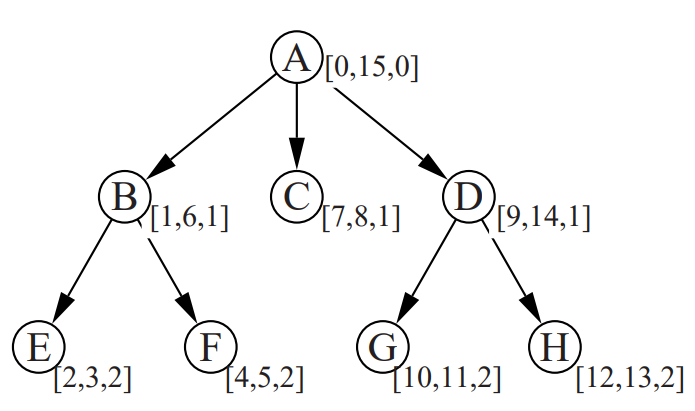
\includegraphics[width=0.4\linewidth]{gripplabeling1}
	\caption{A pre- and postorder labeled tree with depth information.}
	\label{fig:gripplabeling1}
\end{figure}
\begin{claim}
	Given two nodes $u$ and $v$, $u\rightarrow v \Leftrightarrow u_{pre} < v_{pre} < u_{post}$.
\end{claim}
\begin{proof}
	If $u\rightarrow v$, then $u$ must be the ancestor of $v$. So obviously, $u_{pre} < v_{pre}$. Notice that only one counter is used to calculate pre- and postorder values, then obviously, $v_{pre} < u_{post}$. We can observe this property in the example shown in figure \ref{fig:gripplabeling1}.
\end{proof}
The above method is based on a tree, but in most cases, a DAG is not a tree. GRIPP is created to cope with more general cases. GRIPP uses special index table named \textbf{IND(G)}.

\begin{enumerate}
	\item \textbf{Index Construction}
	
	Steps:
	\begin{itemize}
		\item Choosing the root node as the starting node, traverse the tree.
		\item If an arbitrary node $v$ is visited at the first time, push the triple $(v_{pre}, v_{post}, v_{depth})$ to $IND(G)$ as a \textbf{tree instance} and traverse in subtrees.
		\item If an arbitrary node $v$ is visited again, push the triple to $IND(G)$ as a \textbf{non-tree instance} but not traverse.
	\end{itemize} 
	
	\begin{definition}{(Tree and non-tree instances)} 
	Let $IND(G)$ be the index table of graph $G=(V,E)$. Let $v\in V$ be a node of G and $v'$ be an instance of $v$ in $IND(G)$. $v'$ is a tree instance of $v$, iff it was the first instance created for $v$ in $IND(G)$. Otherwise $v'$ is a non-tree instance of v.
	\end{definition}
 	In the following, we refer to any instance in $IND(G)$ of a node $v$ as $v'$, to a tree instance as $v^T$, and to a non-tree instance as $v^N$. The set of tree instances in $IND(G)$ is $I^T$ and the set of non-tree instances is $I^N$. In analogy, the set of tree edges is $E^T$ and the set of non-tree edges $E^N$.
	
	\begin{example}
		Figure \ref{fig:grippexam1} shows a graph and Figure \ref{fig:grippexam1ind} shows its index table, resulting from a traversal in lexicographic order of node labels. Nodes A and B have two instances in $IND(G)$ because they have two incoming edges.
	\end{example}
	
	\begin{figure}[H]
		\centering
		\subfigure[A graph G]{
			\begin{minipage}[t]{0.48\textwidth}
				\centering
				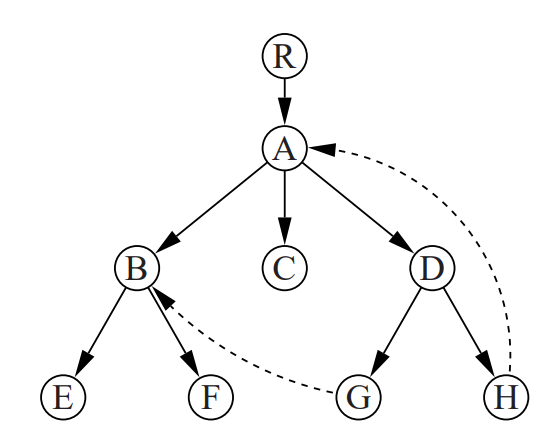
\includegraphics[width=0.7\linewidth]{grippexam1}
				\label{fig:grippexam1}
		\end{minipage}}
		\subfigure[The index table IND(G)]{
			\begin{minipage}[t]{0.48\textwidth}
				\centering
				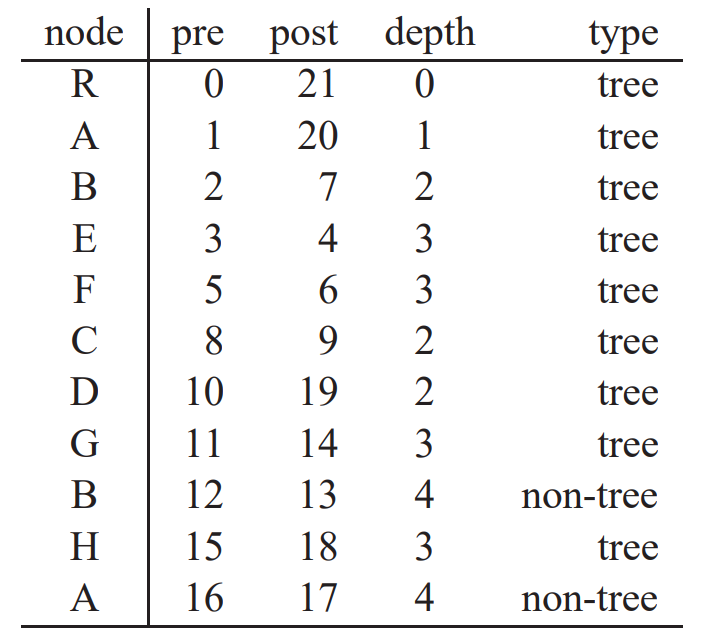
\includegraphics[width=0.7\linewidth]{grippexam1(ind)}
				\label{fig:grippexam1ind}
		\end{minipage}}
		\caption{Graph G and its GRIPP index table IND(G). Solid lines in the graph
			represent tree edges, dashed lines are non-tree edges.}
	\end{figure}
	\begin{claim}
		The index construction takes $O(n + m)$ time.
	\end{claim}
	\begin{proof}
		Done through \textbf{depth first traversal}, taking $O(n + m)$ time.
	\end{proof}
	\item \textbf{Query processing}
	
	\begin{definition}{(Order Tree)}
		Let $G=(V,E)$ and let $IND(G)$ be its index table. The order tree, $O(G)$, is a tree that contains all instances of $IND(G)$ as nodes connected by
		all edges of $G$.
	\end{definition}
	\begin{figure}[H]
		\centering
		\includegraphics[width=0.3\linewidth]{"order tree"}
		\caption{Pre-/ postorder plane for GRIPP index table from Figure \ref{fig:grippexam1ind}. Dotted lines indicate O(G). Non-tree instances are displayed in gray.}
		\label{fig:order-tree}
	\end{figure}
	\begin{definition}{(Reachable Instance Set)}
		Let $v\in V $ be a node of graph $G$ and $v^T \in IND(G)$ its tree instance. The reachable instance set of $v$, written $RIS(v)$, is the set of all instances that are reachable from $v^T$ in $O(G)$, i.e., have a preorder value in $[v_{pre}^T, v_{post}^T]$.
	\end{definition}
	\begin{definition}{(Hop Node)}
		Let $v$, $w\in V$ and $w^N$ be a non-tree instance of $w$. If $w^N \in RIS(v)$ then $w$ is called a hop node for $v$.
	\end{definition}
	\begin{algorithm}[H]
		\caption{ Function to answer $reach(v, w)$ using the GRIPP index.}  
		\label{alg:gripp}
		used\_hops $\leftarrow \varnothing$\;
		used\_stops $\leftarrow \varnothing$\;
		
		\eIf{$w\in RIS(v)$}{
			return true\;
		}
		{
			$used\_hops\leftarrow used\_hops\cup (v)$\;
			\eIf{$v \in \text {STOP\_NODES}$}
			{
				$used\_stops \leftarrow used\_stops\cup(\mathrm{v})$\;
				return false\;
			}
			{
				\While{$non\_tree\_inst\leftarrow nextStop(RIS(v))$}{
					$tree\_inst\leftarrow getTreeInst (non\_tree\_inst)$\;
					\If{$reachability(tree\_inst, w)$}{
						return true\;
					}
				}
				\If{$isInRIS(v, used\_stops)$}
				{
					return false\;
				}
				$\mathrm{H}_{1}\ldots\mathrm{H}_{n}\leftarrow getUsedHopsInRIS(v)$\;
				$non\_tree\_instances\leftarrow getNonTreeInst(RIS(v)\backslash RIS(H_1) \backslash ... \backslash RIS(H_n))$\;
				\ForEach{$non\_tree\_inst\in non\_tree\_instances$}
				{
					$tree\_inst\leftarrow getTreeInst(non\_tree\_inst)$\;
					\If {$!hasChildren(tree\_inst)$} {continue\;}
					
					\If{$tree\_inst\in used\_hops$}
					{continue\;}
					
					\If{$isInRIS(tree\_inst, used\_hops)$}
					{continue\;}
					
					\If{$reachability(tree\_inst, w)$}{
						return true\;
					}
				
					\If{$isInRIS(tree\_inst, used\_hops)$}
					{return false\;}
				}
				return false\;
			}
		}
	\end{algorithm}  
	Given two nodes $u$ and $v$, if we want to know whether $u\rightarrow v$. 
	
	Steps of query:
	\begin{itemize}
		\item Check whether $v\in RIS(u)$.
		\item If not, check all hop nodes and recursively check their reachable instance sets.
	\end{itemize}
	\begin{claim}
		The query would take $O(m-n)$ time in the worst cases.
	\end{claim}
	\begin{proof}
		In the worst cases, the query would traverse all the hop nodes. Each hop node is derived from a non-tree edge, the number of which is $O(m-n)$. Therefore, the query would take $O(m-n)$ time.
	\end{proof}
	\begin{claim}
		The efficiency of query would be improved by pruning.
	\end{claim}
	GRIPP keeps a list $U$ of all nodes that were used to retrieve a
	reachable instance set, i.e., the start node and the hop nodes. Assume we have found a new hop node $h$. Whether $RIS(h)$ should be considered depends on the location of the tree instance $h^T$ of $h$ relative to the tree instances of nodes in $U$.
	Here are the four possibility position of $h^T$ and $u^T, u\in U$.
	\begin{figure}[H]
	\centering
	\subfigure[$h^T equals\ u^T$]{
		\begin{minipage}[t]{0.4\textwidth}
			\centering
			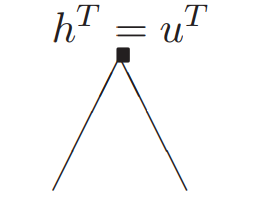
\includegraphics[width=0.6\linewidth]{GRIPP4pos1}
			\label{fig:gripp4pos1}
	\end{minipage}}
	\subfigure[$h^T successor\ of\ u^T$]{
		\begin{minipage}[t]{0.4\textwidth}
		 	\centering
			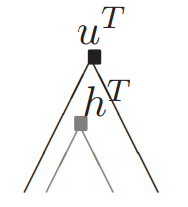
\includegraphics[width=0.5\linewidth]{GRIPP4pos2}
			\label{fig:gripp4pos2}
	\end{minipage}}
	\subfigure[$h^T ancestor\ of\ u^T$]{
		\begin{minipage}[t]{0.4\textwidth}
	 	 	\centering
			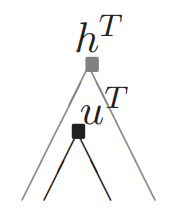
\includegraphics[width=0.5\linewidth]{GRIPP4pos3}
			\label{fig:gripp4pos3}
	\end{minipage}}
	\subfigure[$h^T sibling\ of\ u^T$]{
	\begin{minipage}[t]{0.4\textwidth}
		\centering
		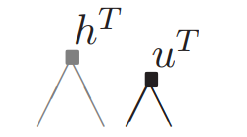
\includegraphics[width=0.7\linewidth]{GRIPP4pos4}
		\label{fig:gripp4pos4}
	\end{minipage}}
	\caption{Possible locations of $h^T$ of hop node $h$ relative to $u^T$, $u\in U$}
	\end{figure}
	Explanation:
	\begin{enumerate}[(a)]
		\item $h^T$ is equal to the tree instance of any node in $U$;
		\item $h^T$ is the successor if the tree instance of at least one node in $U$;
		\item $h^T$ is ancestor of the tree instance of at least one node in $U$ and neither (a) and (b) is true;
		\item $h^T$ is sibling to the tree instances of all nodes in $U$.
	\end{enumerate}
	\paragraph{Skip Strategy} {
		\begin{itemize}
			\item For case (a) and (b), obviously, $RIS(h) \subseteq RIS(u)$, their is no need to traverse $h$, just skip it;
			\item For case (d), no pruning is possible;
			\item For case (c), we only have to consider
			instances from $RIS(h)$ whose preorder values lie outside the pre- and postorder range of $u^T$.
		\end{itemize}
	}
	\paragraph{Stop Strategy} {
		\begin{definition}{(Stop Node)}
			Let $s\in V$ be a node of graph $G$ and let $RIS(s)$ be its reachable instance set in $O(G)$. $s$ is called a stop node iff all non-tree instances in $RIS(s)$ also have their corresponding tree instances in $RIS(s)$ or are a non-tree instance of $s$.
		\end{definition}
		When we reach the tree instance of a stop node $s$, we only have to check if the target node $v$ is in $RIS(s)$. 
	}
	\item \textbf{Space}
	
	Store the information of nodes and the index table would take $O(n+m)$.
\end{enumerate}

\subsubsection{Optimal Chain Cover}
\begin{definition} {(Chain Cover)}
	Let $C=\{c_1,c_2,…,c_k\}$ the set containing some chains of a given graph $G=(V,E)$. If $\forall u \in V, \exists i:u\in c_i$ and $\forall i \neq j, c_i \cap c_j = \varnothing$, then $C$ is of chain cover of $G$.
\end{definition}
\begin{definition} {(Optimal Chain Cover)}
	A chain cover $C$ with least number of chains is an \textbf{optimal chain cover}.
\end{definition}
\begin{enumerate}
	\item \textbf{Index Construction}
	\begin{claim}
	Optimal Chain Cover ${\leq}_p$ Min-Flow.
	\end{claim}
	Given a graph $G=(V,E)$, we can construct another graph $H=(V',E')$. Any node $v_i$ is presented as a directed edge $(x_i, y_i)$ in $H$. A source node is added
	into $H$ that links to every node with in-degree 0 in $H$, and a sink node is added
	that is linked by every node with out-degree 0 in $H$. Each flow in $H$ corresponds to a chain in $G$. We will get an optimal chain cover by finding the min-flow from the source node to the sink node(such that every edge $(x_i, y_i)\in E'$ has a positive flow). 
	
	Such method can be solved through \textbf{Ford Fulkerson’s algorithm} in $O(n^3)$ time.
	\item \textbf{Space}
	
	For each node $v_i\in G$, it is denoted a \textbf{chaincode}, which is a list of pairs: ${(1, p_{i, 1}), (2, p_{i, 2}), ..., (k, p_{i,k})}$. Each pair $(j, p_{i,j})$ means that the node $v_i$ can reach any node $s$ from the position $p_{i,j}$ in the $j$-th chain. If $v_i$ cannot reach any node in the $j$-th chain, then $p_{i,j} = +\infty$. The chain cover index contains chaincode($v_i$) for every node $v_i$ in $G$.
	The chaincode will take $O(nk)$ space in total(where $k$ is the number of chains). 
	\item \textbf{Query processing}
	
	If the number of chain $k$ is small enough to store the index into a 2D table, then the query yields $O(1)$. Otherwise storing it into lists and indexing the lists yields $O(logn+k)$ query time.
	
\end{enumerate}

\subsubsection{2 Hop-Cover}
In a \textbf{2-hop cover}, a node $u$ in G is assigned to a 2-hop code, $2hopcode(u)=(L_{in}(v),L_{out}(v))$, where $L_{in}(v)$ and $L_{out}(v)$ are subsets of the nodes in $G$\cite{ref5}.

\paragraph{Query}  {
	A reachability query $u\rightarrow v$ is to be answered true iff $P_{2hop}(2hopcode(u),2hopcode(v)) = L_{out}(v)\cap L_{in}(v)\neq \varnothing$.
}
\paragraph{Main idea} {
	If we take one node $u$ as a center node, for all nodes $w$ in the ancestors of $u$(denoted as $ancs(u)$) and all nodes $v$ in the descendants of $u$(denoted as $desc(u)$), $w\rightarrow v$.
}
\begin{claim}
	Finding a minimum 2-hop cover in a graph is \textbf{NP hard}. 
\end{claim}

\paragraph{Approximate Solution}  {
	Greedily pick the node with the highest compression as a center node. The approximate ratio is $\log{n}$.
}

\begin{enumerate}
	\item Index Construction: Complicated and costly $O(n^3|T_C|)=O(n^5)$.
	\item Query processing: $O(m^{1/2})$
	\item Space: $O(nm^{1/2})$
\end{enumerate}

\subsection{Index-free algorithms}
Index-free algorithms are various. \textbf{Traversal}, \textbf{Heuristic Search}, and \textbf{Random Walks} are two common algorithms.
\subsubsection{Naïve Traversal}
DFS/BFS can solve reachability problem without index, saving lots of space. But such methods are naïve for large-scale graph, for the methods will traverse the graph which in the worst cases yields $O(n+m)$. Though DFS can be optimized by pruning, but it's still not practical for large-scale graph.
\subsubsection{Bidirectional Search(Two-end BFS)}
Bidirectional search is a graph search algorithm which find smallest path form source to goal vertex. It runs two simultaneous search:

\begin{itemize}
	\item Forward search form source/initial vertex toward goal vertex
	\item Backward search form goal/target vertex toward source vertex
\end{itemize}

Bidirectional search replaces single search graph(which is likely to grow exponentially) with two smaller sub graphs – one starting from initial vertex and other starting from goal vertex. The search terminates when \textbf{two graphs intersect}.

In many cases it is faster, it dramatically reduce the amount of required exploration. Suppose if branching factor of tree is $b$ and distance of goal vertex from source is $d$, then the normal BFS/DFS searching complexity would be $O(b^d)$. On the other hand, if we execute two search operation then the complexity would be $O(b^{\frac{d}{2}})$ for each search and total complexity would be $O(b^{\frac{d}{2}}+b^{\frac{d}{2}})=O(b^{\frac{d}{2}})$ which is far less than $O(b^d)$.
\subsubsection{Heuristic search}
Heuristic algorithms, such as $A^*$, are used to improve the efficiency.

$A^*$ selects the path that minimizes $f(n)=g(n)+h(n)$, where $n$ is the last node on the path, $g(n)$ is the cost of the path from the start node to $n$, and $h(n)$ is a heuristic function that estimates the cost of the cheapest path from n to the goal.
Typical implementations of $A^*$ use a priority queue to perform the repeated selection of minimum (estimated)
cost nodes to expand. This priority queue is known as the open set or fringe. At each step of the algorithm, the node with the lowest $f(x)$ value is removed from the queue, the $f$ and $g$ values of its neighbors are updated accordingly, and these neighbors are added to the queue. The algorithm continues until a goal node has a lower $f$ value than any node in the queue (or until the queue is empty).

If the heuristic function $h$ is admissible, meaning that it never overestimates the actual minimal cost of reaching the goal, then $A^*$ is itself admissible (or optimal) if we do not use a closed set. If a closed set is used, then $h$ must also be monotonic (or consistent) for $A^*$ to be optimal. This means that for any pair of adjacent nodes $x$ and $y$, where $d(x,y)$ denotes the length of the edge between them, we must have:
$$
h(x) \leq d(x, y)+h(y)
$$

This ensures that for any path $X$ from the initial node to $x$:
$$
L(X)+h(x) \leq L(X)+d(x, y)+h(y)=L(Y)+h(y)
$$
where $L$ is a function that denotes the length of a path, and $Y$ is the path $X$ extended to include $y$. In other words, it is impossible to decrease (total distance so far + estimated remaining distance) by extending a path to include a neighboring node.

Monotonicity implies admissibility when the heuristic estimate at any goal node itself is zero, since (letting $P = \left(f, v_{1}, v_{2}, \ldots, v_{n}, g\right)$ be a shortest path from any node $f$ to the nearest goal $g$):

$$
h(f) \leq d\left(f, v_{1}\right)+h\left(v_{1}\right) \leq d\left(f, v_{1}\right)+d\left(v_{1}, v_{2}\right)+h\left(v_{2}\right) \leq \ldots \leq L(P)+h(g)=L(P)
$$

The time complexity of $A^*$ depends on the heuristic. In the worst case of an unbounded search space, the number of nodes expanded is exponential in the depth of the solution (the shortest path) $d$: $O(bd)$, where $b$ is the branching factor (the average number of successors per state).

\subsubsection{ARROW}
The index-based algorithms work well when the graph is not updated or updated infrequently, while in practical applications the graph is usually large-scale and dynamic(such as social networks). \textbf{ARROW}(Approximating Reachability using Random-walks Over Web-scale graphs)\cite{ref6} has been created to better cope with dynamic networks.

\begin{definition}{(Graph Diameter)}
	The diameter of graph is the maximum distance between the pair of vertices.
\end{definition}

\paragraph{Main Idea}  {
	Given a reachability query $(u,v)$ on a graph snapshot(since the grpah is \textbf{dynamic}) $G_t(V_t,E_t)$ at time $t$, with $|V_n| = n$, ARROR constructs two sets of `stops', $F(u) = {s:u\rightarrow s}$	and $B(v) = {t:t\rightarrow v}$. ARROW answers TRUE iff $F(u)\cap B(v)\neq \varnothing$. It's kind of like 2-Hop labeling, but notice that ARROW stores no index. The sets $F(u)$ and $B(v)$ are constructed through \textbf{random walks}.
}

\paragraph{Random Walks}  {
	ARROR constructs $r=c_{\text{numWalks}} \times \sqrt[3]{n^{2} \ln n}$ random walks, where $c_{\text{numWalks}}$ is a parameter to be set. Each walk is of length $l=c_{\text {walkLength }} \times \text { diam }$ from $u$ on $G_t$, where $diam$ is the diameter of the graph and $c_{\text{walkLength}}$ is the diameter to be set.
}

\begin{algorithm}[H]
	\caption{ARROW}  
	\label{alg:arrow}  
	\textbf{Algorithm} ARROW($G_t$, $u$, $v$)
	
	$wL\leftarrow c_\text{walkLength}\times diam$\;
	$F(u)\leftarrow B(v)\leftarrow \varnothing$\;
	\For{$w$ in $1...c_\text{numWalks}\times \sqrt[3]{n^2\ln(n)}$}{
		currentNode $\leftarrow u$\;
		\For{$s$ in $1...wL$}{
			neighbour $\leftarrow$ random neighbour of currentNode\;
			$F(u)=F(u)\cup$ \{neighbour\}\;
			currentNode $\leftarrow$ neighbour\;
		}
	}
	\textbf{return} $F(u)\cap B(v)\neq \varnothing$\;
\end{algorithm}  

\paragraph{Theoretical bound on number of walks} {
	\begin{claim}
		$r=c_{\text{numWalks}} \times \sqrt[3]{n^{2} \ln n}$ is a pessimistic upper bound on the number of walks required to obtain the correct anwser with high probability.
	\end{claim}
	\begin{proof}
		Given a strongly connected graph $G$ with vertex set $V$, such that $|V| = n$, let the random walk conducted on the directed edges in the forward direction have transition matrix $\overrightarrow{P}$ and stationary distribution $\overrightarrow{\pi}$, and the random walk on the directed edges traversed in the reverse direction have transition matrix $\overleftarrow{P}$ and stationary distribution $\overleftarrow{\pi}$. Given two integers $k,t^*>0$, consider two collections of random walks of length $t^*$, $\{(X^i_t)_{t\leq0},X_0^i=x:1\leq i\leq k\}$ started from $x\in V$ conducted according to $\overrightarrow{P}$ and $\{(Y^i_t)_{t\leq0},Y_0^i=y:1\leq i\leq k\}$ started from $y\in V$ conducted according to $\overleftarrow{P}$.
		
		Futher define $S_{x}=\left\{X_{t^{*}}^{i}: 1 \leq i \leq k\right\}, S_{y}=\left\{Y_{t^{*}}^{i}: 1 \leq i \leq k\right\}$
		
		If 
		$$t^{*} \geq \max \left\{t_{\operatorname{mix}}^{\overrightarrow{P}}\left(\frac{1}{\sqrt{2} n}\right), t_{\operatorname{mix}}^{\overleftarrow{P}}\left(\frac{1}{\sqrt{2} n}\right)\right\}$$
		then $P\left\{S_{x} \cap S_{y} \neq \varnothing\right\} \geq 1-1 / n$ if
		$$k \geq k^{*}=\left\{\frac{16 n^{2} \ln n}{(\alpha(\overrightarrow{\pi}, \overleftarrow{\pi}))^{2}}\right\}^{\frac{1}{3}}$$ 
		whenever
		$$k^{*} \cdot\left(\max \{\max \{\mu(i): 1 \leq i \leq n\}, \max \{\nu(i): 1 \leq i \leq n\}\}+\frac{1}{2 n}\right)<1$$
		where 
		$$\alpha(\overrightarrow{\pi}, \overleftarrow{\pi})=n\left(\sum_{i=1}^{n} \max \left\{0, \overrightarrow{\pi}(i)-\frac{1}{2 n}\right\} \cdot \max \left\{0, \overleftarrow{\pi}(i)-\frac{1}{2 n}\right\}\right)$$
		In particular, if $\alpha(\overrightarrow{\pi}, \overleftarrow{\pi})$ is a constant then $k^{*}=\theta\left(\sqrt[3]{n^{2} \ln n}\right)$
	\end{proof}
}
\paragraph{Diameter estimation}  {
	Determine the exact diameter of a given graph is usually very costly in practical application, so ARROW uses an approximate method instead: Selecting the longest distance recorded across 10 rounds of BFS from randomly selected nodes on the given graph.
}
\paragraph{The problem of escape from SCCs}  {
	Assume that a walk begun from a vertex $v$ and run for $t$ steps stays within its SCC with probability $p(t,v)$. If we conduct $c \sqrt[3]{n^{2} \ln n}$ independent walks for some appropriately chosen $c$, then we can argue by Chernoff bounds that $c^{\prime} \sqrt[3]{n^{2} \ln n}$ of them stay within the SCC with probability $1-1 / n$ if
	$$
	p(t, v) \geq \frac{\ln n}{\sqrt[3]{n^{2} \ln n}}
	$$
	This bound decreases with n faster than $n^{-2/3}$ and, so, is a relatively modest requirement, especially from those vertices that are deep within the SCC.
}
\paragraph{Complexity} {
	The sizes of sets $F(u)$ and $B(v)$, and the time taken to construct and intersect them are all $r\cdot l$, where $r$ is the number of random walks and $l$ is the length of walks, as defined in Section II-A. Therefore, query answering time is $\mathcal{O}\left(\sqrt[3]{n^{2} \ln n} \cdot \text { diam }\right)$
}

\subsubsection{Other methods}
In practical application, we may be interested in not only the information of reachability, but also the distance of two nodes. So usually, reachability is determined at the same time when solving the shortest path problem. This is very common in the application of map, such as Google Map.

Table \ref{table:shortest-path} shows some mainstream shortest-path algorithms.
\begin{table}[H]
	\centering
	\caption{\newline \ Three mainstream shortest-path algorithm.}
	\begin{tabular}{l|l|l}
		\toprule
		Method & Time Complexity & Space Complexity  \\ \midrule
		Dijkstra&  $O(V+E\log{V})$   &$O(V^2)$  \\ \midrule
		Floyd&   $O(V^3)$      & $O(V^2)$ \\ \midrule
		Bellman Ford& $O(VE)$(average) and $O(V^3)$(worst)&$O(V)$\\ \bottomrule
	\end{tabular}
	\label{table:shortest-path}
\end{table}

\section{Practical Algorithm}
A graph can be categoried into dynamic(frequently updated) graph and static(infrequently updated). For the static one, the typically best method is to construct an index(which will take a relatively long time in construction but save huge amount of time in query), while for the dynamic one, traversal or random walk is considered practical.
\subsection{Static(infrequently updated) Graph}
We have introduced lots of index-based algorithms above, like `Optimal tree cover', `2-Hop labeling', etc, in which `GRIPP' excels.

As is displayed in Table \ref{table:algorithms}, for GRIPP, its index construction yields $O(n+m)$, its query yields $O(m-n)$, and it needs $O(n+m)$ space for index. If given a dense graph($m\approx n^2$), the construction and query will both yield $O(n^2)$. If given a sparse graph($m\approx kn$), the query will yield $O(n)$. So GRIPP performs well when given a sparse graph, and is still acceptable given a very dense graph. But its construction time is still too long for a dynamic graph. So it's appropriate for static(infrequently updated) graph(useful in biological analysis), but not for dynamic one like social network.

Fortunately, although graphs are often updated in real time, in many application scenarios we do not need to update graphs frequently to deal with immediate changes.  Facing this kind of application scenario, by pre-establishing indexes (using distributed parallel computing frameworks such as Spark), good query efficiency can be provided.
\begin{figure}[H]
\centering
\subfigure[Average size(tuples)]{
	\begin{minipage}[t]{0.48\textwidth}
		\centering
		\includegraphics[width=0.9\linewidth]{grippexp1}
		\label{fig:grippexp1}
\end{minipage}}
\subfigure[Average time (sec)]{
	\begin{minipage}[t]{0.48\textwidth}
		\centering
		\includegraphics[width=0.9\linewidth]{grippexp2}
		\label{fig:grippexp2}
\end{minipage}}
\caption{Average time and size for the GRIPP index table, Dual Labeling on the component graph, and the transitive closure for synthetic scale-free graphs with 100 \% more edges than nodes.\cite{ref4}}
\end{figure}
\subsection{Dynamic(frequently updated) Graph}
Faced with the problem of accessibility of dynamic graphs, we can often use traversal.  But for a large-scale graph, traversal may traverse all edges and nodes in the worst case, which is unacceptable.  Moreover, in many application scenarios, we often do not need to give a very accurate answer (such as judging whether two people know each other in a social network), so using some approximation or randomization algorithms will greatly improve query efficiency.

ARROW's query time complexity is $O\left(\sqrt[3]{n^{2} \ln n} \cdot \operatorname{diam}\right)$. When given a dense graph($m\approx n^2$), the common BFS/DFS yields $O(m+n)=O(n^2)$. In this case, ARROW's query performs better than BFS/DFS. That is to say, ARROW sacrifices a little accuracy to get better performance. 

The table \ref{table:ARROW} shows the experimental results of some datasets.\cite{ref6} 
\begin{table}[H]
	\centering
	\caption{Dynamic Graph Results (Timeout = 2 hours, $c_{\text {numWalls }}=0.01, c_{\text {walkLength }}=1$)} 
	\setlength{\tabcolsep}{1mm}{
		\begin{tabular}{l|l|l|l|l|l|l|l|c}
		\toprule 
		\textbf{Dataset} & Method& Insert(ms) & Delete(ms) & Query(ms) & Init(ms) & Mem(MB) & Total(ms) & Acurracy \\ \midrule
		Facebook&DAGGER&0.22&90.405&0.1655&446.091&4007.7&8244220&\\
		&ARROW&0.00025&0.00049&0.7868&3.437&12.69&\textbf{674.99}&0.956\\
		&BBFS&0.000192&0.000321&6.8775&0.00016&13.172&4324.954&\\
		&BFS&0.000143&0.00031&18.8432&0.000138&6.809&10286.772&\\ \midrule
		
		Enron&DAGGER&864.27&1.08188&0.0048&604.135&44.04&TIMEOUT&\\
		&ARROW&0.000229&0.000514&0.0468&6.45&18.53&\textbf{2818.158}&1\\
		&BBFS&0.000263&0.000627&1.0011&0.00014&18.537&3091.943&\\
		&BFS&0.00021&0.00051&2.1536&0.00027&8.631&3470.022&\\ \midrule  
		
		Epinions&DAGGER&55.7711&71.0257&2.577&1786.1&1453.75&TIMEOUT&\\
		&ARROW&0.000135&0.000191&6.599943&95.166&17.42&\textbf{808.029}&0.998\\
		&BBFS&0.00017&0.00024&14.345296&0.00024&18.086&8198.45&\\
		&BFS&0.00011&0.00013&14.966&0.000086&8.86&8561.26&\\ \midrule
		
		Flickr&DAGGER&NA&NA&NA&TIMEOUT&NA&TIMEOUT&\\
		&ARROW&0.000223&0.000532&285.872&4354.84&415.011&\textbf{45334.908}&0.986\\
		&BBFS&0.000307&0.000703&463.7533&0.00022&470.299&290706.677&\\
		&BFS&0.0002491&0.001004&665.575&0.000149&208.584&405832.625&\\ \bottomrule     
		\end{tabular}
	}
\label{table:ARROW}
\end{table}
\subsection{Improved Heuristic Searching}
Above we introduced the heuristic algorithm $A^*$. While the admissibility criterion of $A^*$ guarantees an optimal solution path, it also means that $A^*$ must examine all equally meritorious paths to find the optimal path. To compute approximate shortest paths, it is possible to speed up the search at the expense of optimality by relaxing the admissibility criterion. Oftentimes we want to bound this relaxation, so that we can guarantee that the solution path is no worse than $(1 + \varepsilon)$ times the optimal solution path. This new guarantee is referred to as $\varepsilon$-admissible.
There are a number of $\varepsilon$-admissible algorithms:
\begin{itemize}
	\item \textbf{Weighted $A*$/Static Weighting's}\cite{ref7} If $h_a(n)$ is an admissible heuristic function, in the weighted version of the $A^*$ search one uses $h_w(n) = \varepsilon h_a(n), \varepsilon > 1$ as the heuristic function, and perform the $A^*$ search as usual (which eventually happens faster than using ha since fewer nodes are expanded). The path hence found by the search algorithm can have a cost of at most $\varepsilon$ times that of the least cost path in the graph.\cite{ref8}
	\item \textbf{Dynamic Weighting}\cite{ref9} uses the cost function $f(n)=g(n)+(1+\varepsilon w(n)) h(n)$, where $$w(n)= \begin{cases}1-\frac{d(n)}{N} & d(n) \leq N \\ 0 & \text { otherwise }\end{cases}$$ 
	and where $d(n)$ is the depth of the search and $N$ is the anticipated length of the solution path.
	\item \textbf{Sampled Dynamic Weighting}\cite{ref10} uses sampling of nodes to better estimate and debias the heuristic error.
	\item $A_{\varepsilon}^{*}$\cite{ref11} uses two heuristic functions. The first is the FOCAL list, which is used to select candidate nodes, and the second hF is used to select the most promising node from the FOCAL list.
	\item $A_{\varepsilon}$\cite{ref12} selects nodes with the function $A f(n)+B h_{F}(n)$, where $A$ and $B$ are constants. If no nodes can be selected, the algorithm will backtrack with the function $C f(n)+D h_{F}(n)$, where $C$ and $D$ are constants.
	\item \textbf{Alpha$A^*$}\cite{ref13} attempts to promote depth-first exploitation by preferring recently expanded nodes. Alpha$A^*$ uses the cost function $f_{\alpha}(n)=\left(1+w_{\alpha}(n)\right) f(n)$, where 
	$$
	w_{\alpha}(n)= \begin{cases}\lambda & g(\pi(n)) \leq g(\tilde{n}) \\ \Lambda & \text { otherwise }\end{cases}
	$$
	where $\lambda$ and $\Lambda$ are constants with $\lambda \leq \Lambda$, $\pi(n)$ is the parent of $n$, and $\tilde{n}$ is the most recently expanded node.  
\end{itemize}
\section{Concluding Remarks}
In practical applications, there are different algorithms dealing with different graphs. We cannot find a universal algorithm that works in all situations. Index-based algorithms are more suitable for static or infrequently updated graphs, and are suitable for application scenarios that require high precision and high query efficiency, such as scientific research and analysis.

There are many index-based algorithms, tree-cover, chain-cover, two-hop cover... We can’t say that a certain algorithm is suitable for all static graphs. Some algorithms are more efficient for dense graphs while some are more efficient for sparse graphs. Some are suitable for large-scale graphs while some are suitable for small-scale graphs. Some are slow to construct but very fast to query while some are very fast to query but very slow to construct. Rather than choosing a fixed algorithm, it is better to heuristically select the most suitable algorithm according to the shape of the graph, the number of nodes, and the density of the graph. To form a unified framework that can deal with different graphs is one of the directions worth studying in the future.

Whether using traditional traversal, heuristic search or random walk can all cope with the real-time dynamic changes of the graph. Although traditional traversal guarentees to determine the reachability between two points, it may traverse all vertices and edges in the worst case. Unfortunately, most of the graphs in reality are very large, and such traversal is unacceptable.

In order to improve efficiency, we usually use heuristic algorithms or random algorithms (random walks) or some approximate algorithms in applications. These algorithms greatly improve the efficiency of query and meet the needs of most applications. (Because in many daily applications, we often don't need 100\% accurate answers.)

Although these algorithms have significantly improved efficiency in most cases, in some cases, the algorithms may degenerate into ordinary traversal algorithms. Moreover, algorithms such as random walk sacrifice a part of accuracy in exchange for higher query efficiency, which may not be applicable in some scenarios with high accuracy requirements. Of course, you can classify queries, by using random walk algorithms for requests that do not require high accuracy, and using DFS/BFS for requests that require high accuracy. 

In reality, graphs are generally very large, and even $O(n)$ algorithms are sometimes unacceptable. However, reasonable application of distributed and parallel computing frameworks, such as Spark, Storm, etc., can improve efficiency by taking the adventage of parallel computation.

Graph is a very interesting data structure. It perfectly abstracts many real systems. People's various researches on graphs have been going on for a long time, and I think these researches will continue to develop endlessly. With the continuous improvement of computing power, the continuous development of technology and the continuous maturity of theories, many things that were considered impossible in the past have become reality. Let me think about it here: judging whether two points are reachable (connected) in a circuit is very simple and very fast. Just use an electric meter to check the resistance at both ends. If the resistance is infinite, it means that the two points are not reachable to each other. This physical judgment is often much faster than a logical judgment. I was wondering whether it is possible to transfer a huge graph from the virtual logical world to the physical world, and judge the reachability in a physical way? Of course this is too whimsical at present, but people 200 years ago would not have thought that I would type these words in front of a high-tech machine.
\newpage

\begin{thebibliography}{References}
	\bibitem{ref1} Yu J X, Cheng J. Graph reachability queries: A survey[M]//Managing and Mining Graph Data. Springer, Boston, MA, 2010: 181-215.
	\bibitem{ref2} Agrawal R, Borgida A, Jagadish H V. Efficient management of transitive relationships in large data and knowledge bases[J]. ACM SIGMOD Record, 1989, 18(2): 253-262.
	\bibitem{ref3} Trißl S, Leser U. GRIPP Indexing and Querying Graphs Based on Pre-and Postorder Numbering[M]. Humboldt-Univ. zu Berlin, 2006.
	\bibitem{ref4} Trißl S, Leser U. Fast and practical indexing and querying of very large graphs[C]//Proceedings of the 2007 ACM SIGMOD international conference on Management of data. 2007: 845-856.
	\bibitem{ref5} D'angelo G, D'emidio M, Frigioni D. Fully dynamic 2-hop cover labeling[J]. Journal of Experimental Algorithmics (JEA), 2019, 24: 1-36.
	\bibitem{ref6} Sengupta N, Bagchi A, Ramanath M, et al. Arrow: Approximating reachability using random walks over web-scale graphs[C]//2019 IEEE 35th International Conference on Data Engineering (ICDE). IEEE, 2019: 470-481.
	\bibitem{ref7} Pohl, Ira (1970). ``First results on the effect of error in heuristic search". Machine Intelligence. 5: 219–236.
	\bibitem{ref8} Pearl, Judea (1984). Heuristics: Intelligent Search Strategies for Computer Problem Solving. Addison-Wesley. ISBN 978-0-201-05594-8.
	\bibitem{ref9} Pohl, Ira (August 1973). ``The avoidance of (relative) catastrophe, heuristic competence, genuine dynamic weighting and computational issues in heuristic problem solving" (PDF). Proceedings of the Third International Joint Conference on Artificial Intelligence (IJCAI-73). 3. California, USA. pp. 11–17.
	\bibitem{ref10} Köll, Andreas; Hermann Kaindl (August 1992). ``A new approach to dynamic weighting". Proceedings of the Tenth European Conference on Artificial Intelligence (ECAI-92). Vienna, Austria. pp. 16–17.
	\bibitem{ref11} Pearl, Judea; Jin H. Kim (1982). ``Studies in semi-admissible heuristics". IEEE Transactions on Pattern Analysis and Machine Intelligence. 4 (4): 392–399. doi:10.1109/TPAMI.1982.4767270. PMID 21869053. S2CID 3176931.
	\bibitem{ref12} Ghallab, Malik; Dennis Allard (August 1983). ``Aε – an efficient near admissible heuristic search algorithm" (PDF). Proceedings of the Eighth International Joint Conference on Artificial Intelligence (IJCAI-83). 2. Karlsruhe, Germany. pp. 789–791. Archived from the original (PDF) on 2014-08-06.
	\bibitem{ref13} Reese, Bjørn (1999). ``AlphA*: An ε-admissible heuristic search algorithm". Archived from the original on 2016-01-31. Retrieved 2014-11-05.
\end{thebibliography} 
\end{document}


